\documentclass[10pt]{beamer}

\usepackage{tikz}
\usepackage{graphicx}
\usepackage{fontspec}
\usepackage{hyperref}
\usepackage[absolute,overlay]{textpos}
\usepackage{emoji}

\graphicspath{ {./src/} }

\usefonttheme{professionalfonts}
\usefonttheme{serif}
\setmainfont{DejaVuSansMono}
\setmonofont{DejaVuSansMono-Bold}

\usetheme{Berlin}
\usecolortheme{beaver}

\hypersetup{
    colorlinks=true,
    linkcolor=blue,
    filecolor=magenta,
    urlcolor=cyan,
}


\title{IISC/CTF: replme}
\subtitle{Review of Enowars 8}
\author{Jacob Bachmann}

\institute
{
  SecT\\
  TU Berlin
}

\logo{
	
\includegraphics[scale=0.07]{sect-logo}
}

\begin{document}

\frame{\titlepage}

\begin{frame}
	\begin{center}
		\LARGE{\texttt{About service: replme}}
	\end{center}
\end{frame}

\begin{frame}
	\frametitle{About service: replme}
	\begin{itemize}
		\item<1-> Clone of \href{http://replit.com}{replit.com}
		\item<2-> Provides "DEVENVs" in browser
		\item<3-> Provides "REPLs" in browser
	\end{itemize}
\end{frame}

\begin{frame}
	\begin{center}
		\LARGE{\texttt{DEMO}}
	\end{center}
\end{frame}

\begin{frame}
	\begin{center}
		\LARGE{\texttt{Architecture}}
	\end{center}
\end{frame}

\begin{frame}
	\frametitle{Architecture}
	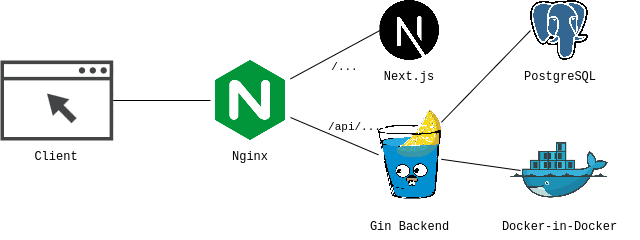
\includegraphics[scale=.45]{arch.drawio}
\end{frame}

\begin{frame}
	\begin{center}
		\LARGE{\texttt{Vuln 1: Path traversal}}
	\end{center}
\end{frame}

\begin{frame}
	\frametitle{Vuln 1: Path traversal}
	\begin{itemize}
		\item<1-> Flagstore is file in devenv
		\item<2-> Devenv files are stored in FS (docker volume)
		      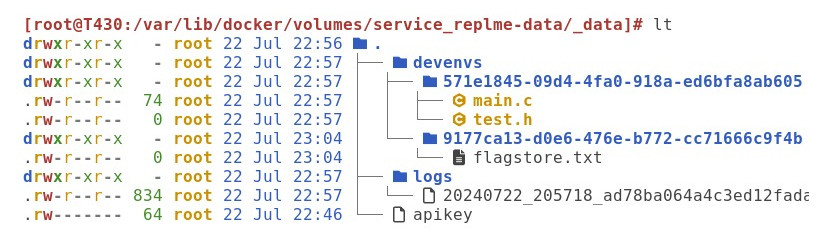
\includegraphics[scale=1.4]{volume-border}
		\item<3-> /api/devenv/\{571..\}/files/flagstore.txt \\
		      \ \ \ \ ?uuid=\{571..\}\%2F..\%2F\{917..\}
	\end{itemize}
\end{frame}

\begin{frame}
	\frametitle{Vuln 1: Path traversal}
	\begin{minipage}{0.39\linewidth}
		\begin{figure}
			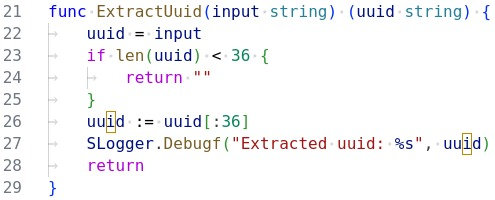
\includegraphics[scale=0.25]{extract-uuid}
			\caption{service/backend/util/encoding.go}
		\end{figure}
	\end{minipage}
	\hspace{0.03\linewidth}
	\begin{minipage}{0.5\linewidth}
		\begin{figure}
			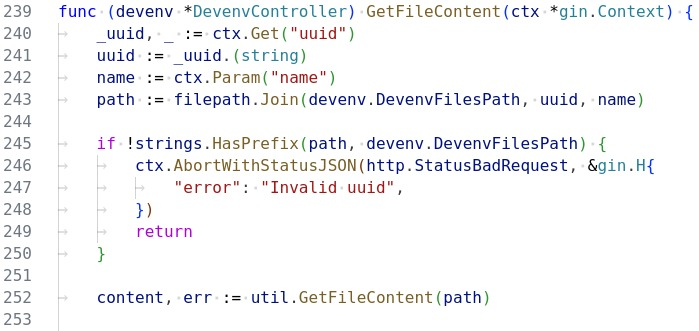
\includegraphics[scale=0.25]{get-file-content}
			\caption{service/backend/controller/devenv.go}
		\end{figure}
	\end{minipage}
\end{frame}

\begin{frame}
	\begin{center}
		\LARGE{\texttt{Vuln 2: 2nd preimage}}
	\end{center}
\end{frame}

\begin{frame}
	\frametitle{Vuln 2: 2nd preimage}
	\begin{itemize}
		\item<1-> Flagstore is file in FS of REPL
		\item<2-> Identifier of REPLs is CRC(username)
		\item<3-> CRC is no cryptographically secure hash func
	\end{itemize}
	\pause
	\pause
	\begin{align*}
		h(a) = a\ \%\ p
	\end{align*}
	\begin{itemize}
		\item<4-> Calculate deltas, such that: \\
		      CRC(username) == CRC(username+delta) \\
	\end{itemize}
	\pause
	\pause
	\begin{align*}
		h(a\oplus\Delta) & =(a\oplus b\cdot p)\ \%\ p \\
		                 & =a\ \%\ p                  \\
	\end{align*}
\end{frame}

\begin{frame}
	\begin{center}
		\LARGE{\texttt{Vuln 3: RCE (Bonus)}}
	\end{center}
\end{frame}

\begin{frame}
	\frametitle{Vuln 3: RCE (Bonus)}
	\begin{itemize}
		\item<1-> Server on REPLs exposes register endpoint
		\item<2-> Endpoint secured by apikey \\
		      http://\{ip\}:\{port\}/api/\{apikey\}/auth/register
		\item<3-> Password is not sanitized
	\end{itemize}
	\pause
	\pause
	\pause
	\begin{figure}
		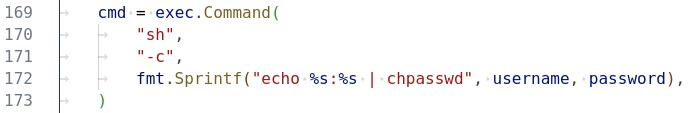
\includegraphics[scale=.4]{register}
		\caption{service/image/service/user.go}
	\end{figure}
\end{frame}

\begin{frame}
	\begin{center}
		\LARGE{\texttt{DEMO}}
	\end{center}
\end{frame}

\begin{frame}
	\begin{center}
		\LARGE{\texttt{What worked}}
	\end{center}
\end{frame}

\begin{frame}
	\frametitle{What worked}
	\begin{itemize}
		\item<1-> Service stable
		\item<2-> SLA was suprisingly good
		\item<3-> People had fun
	\end{itemize}
	\pause
	\pause
	\begin{figure}
		
\includegraphics[scale=.018]{replme-performance}
	\end{figure}
\end{frame}

\begin{frame}
	\begin{center}
		\LARGE{\texttt{What did'nt work}}
	\end{center}
\end{frame}

\begin{frame}
	\frametitle{What did'nt work}
	\begin{itemize}
		\item<1-> Unintended vuln
		\item<2-> Performance issues due to strict timeout
		\item<3-> CORS ❤️
		\item<4-> proxy.prod.bambi.ovh blacklisted
		\item<5-> CRC unexploited
	\end{itemize}
\end{frame}

\begin{frame}
	\begin{center}
		\LARGE{\texttt{Feedback}}
	\end{center}
\end{frame}

\begin{frame}
	\frametitle{Feedback}
	\begin{itemize}
		\item<1-> "the return bug was truly evil btw"
		\item<2-> "i wanted to do that, but i missed the crypto knowledge"
		\item<3-> "exploitation wasn't simple even with this unintended bug though, so it was a fun task"
	\end{itemize}
\end{frame}

\begin{frame}
	\begin{center}
		\LARGE{\texttt{Lessons learned}}
	\end{center}
\end{frame}

\begin{frame}
	\frametitle{Lessons learned}
	\begin{itemize}
		\item<1-> Stay calm and take the time to think
		\item<2-> Do not get lost in details
	\end{itemize}
\end{frame}

\begin{frame}
	\begin{center}
		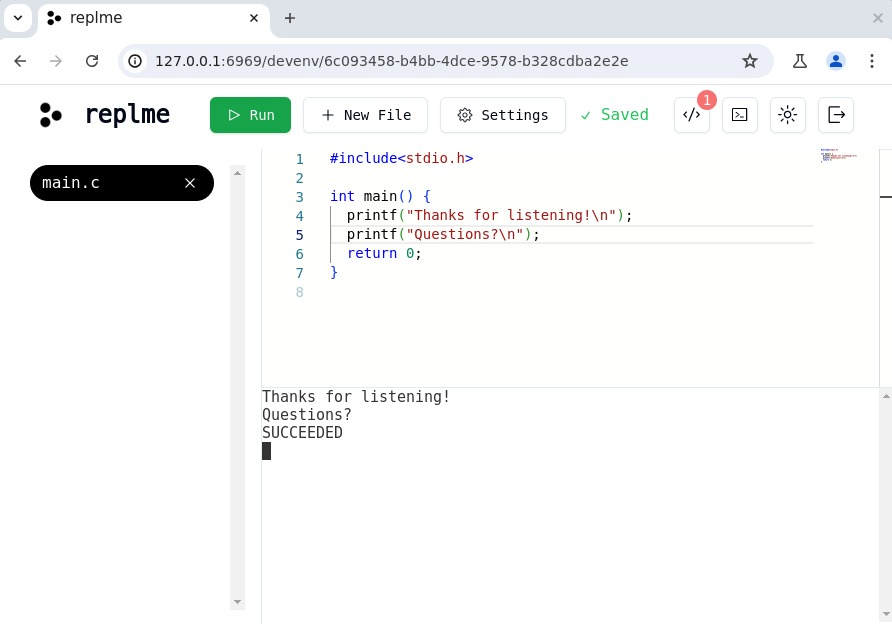
\includegraphics[scale=0.29]{thanks}
	\end{center}
\end{frame}

\end{document}
